 \documentclass{article}

% preambulo:
\usepackage[utf8]{inputenc}
% caracteres utf8 (tildes, enie) sin tener que usar comandos

\usepackage[spanish, es-tabla, es-nodecimaldot]{babel} 
% texto automatico en espaniol
% "tabla" en vez de "cuadro"
% no reemplaza puntos decimales por comas

%% NO AGREGAR PAQUETES ANTES DE ESTO, ES IMPORTANTE QUE BABEL ESTE PRIMERO

%%%%%%%%%%%%%%%%%%%%%%%%%%%%%%%%%
%% PAQUETES EXTRA %%%%%%%%%%%%%%%
%%%%%%%%%%%%%%%%%%%%%%%%%%%%%%%%%

\usepackage{subfiles}

%nuevo
\usepackage[notransparent]{svg}
%

\usepackage{amsmath} % PAQUETES DE MATEMATICA
\usepackage{amsfonts}
\usepackage{amssymb}

%puse esta cosa nueva---
\usepackage{csvsimple}

%-----
\usepackage{steinmetz} % comando \phase{}
\usepackage{units} % permite usar nicefrac
\usepackage{graphicx} % importar imagenes
\usepackage{float} % posicion H para floats
\usepackage[colorinlistoftodos]{todonotes}


\usepackage[a4paper, total={6in, 8in}]{geometry} 
% margenes correctos en subarchivos

\setlength{\parindent}{10pt}			%cuanta sangria al principio de un parrafo
\usepackage{indentfirst}				%pone sangria al primer parrafo de una seccion

\usepackage{listings}

\usepackage{color}

\definecolor{codegreen}{rgb}{0,0.6,0}
\definecolor{codegray}{rgb}{0.5,0.5,0.5}
\definecolor{codepurple}{rgb}{0.58,0,0.82}
\definecolor{backcolour}{rgb}{0.95,0.95,0.92}
 
\lstdefinestyle{mystyle}{
    backgroundcolor=\color{backcolour},   
    commentstyle=\color{codegreen},
    keywordstyle=\color{magenta},
    numberstyle=\tiny\color{codegray},
    stringstyle=\color{codepurple},
    basicstyle=\footnotesize,
    breakatwhitespace=false,         
    breaklines=true,                 
    captionpos=b,                    
    keepspaces=true,                 
    numbers=left,                    
    numbersep=5pt,                  
    showspaces=false,                
    showstringspaces=false,
    showtabs=false,                  
    tabsize=2
}
 
\lstset{style=mystyle}

%%%%%%%%%%%%%%%%%%%%%%%%%%%%%%%%%%%%%%%%%%%%%%%%%%%%%%%%%%%
%% NO AGREGAR PAQUETES DESPUES DE ESTO, ES IMPORTANTE QUE HYPERREF ESTE ULTIMO
\usepackage[hidelinks]{hyperref} % hipervinculos sin cajitas rojas
\usepackage{bm}


\usepackage{fancyhdr}

\geometry{top=2.5cm, bottom=2.0cm, left=2.25cm, right=2.25cm}

\lhead{Sistemas de Control 22.85}
\chead{TP4 - Control Carrito}
\rhead{ITBA}
\renewcommand{\headrulewidth}{1pt}
\renewcommand{\footrulewidth}{1pt}
\pagestyle{fancy}


\begin{document}

%\newgeometry{} % margenes default para la caratula
% caratula:
\begin{titlepage}
\newcommand{\HRule}{\rule{\linewidth}{0.5mm}}
\center
\mbox{\textsc{\LARGE \bfseries {Instituto Tecnol\'ogico de Buenos Aires}}}\\[1.5cm]
\textsc{\Large 22.85 - Sistemas de Control}\\[0.5cm]


\HRule \\[0.6cm]
{ \Huge \bfseries Trabajo de Laboratorio N$^{\circ}$4: Control de Carrito mediante controlador PID}\\[0.4cm] % Title of your document
\HRule \\[1.5cm]


{\large

\emph{Grupo 1}\\
\vspace{3px}

\begin{tabular}{lr} 	
\textsc{M\'aspero}, Martina  & 57120 \\
\textsc{Mestanza}, Joaqu\'in Mat\'ias  & 58288 \\
\textsc{Nowik}, Ariel Santiago  & 58309 \\
\textsc{Panaggio Venerandi}, Guido Martin  & 56214 \\
\textsc{Parra}, Roc\'io  & 57669 \\
\textsc{Regueira}, Marcelo Daniel  & 58300 \\

\end{tabular}

\vspace{20px}

\emph{Profesor}\\
\vspace{3px}
\textsc{Nasini}, V\'ictor Gustavo\\ 	
\vspace{100px}

\begin{tabular}{ll}

Presentado: & 27/11/2019\\

\end{tabular}

}

\vfill

\end{titlepage}


% indice:
\tableofcontents
\newpage

\section{PID: Introducción teórica}
Los controladores PID (proporcional, integrador y derivativo) proveen un control de lazo empleando feedback que es utilizado en la industria del control.
Un controlador PID calcula el error e(t) como la diferencia entre el setpoint (deseada) y una variable medida del proceso (la salida de la planta).


\begin{figure}[H]
\centering
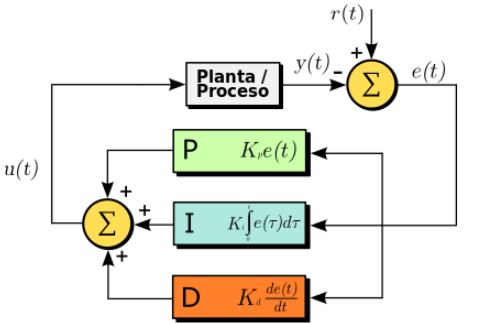
\includegraphics[width=0.5\linewidth]{images/PID.jpg}
\caption{Controlador PID: Esquema}
\label{fig:PID}
\end{figure}

Como se puede observar en la figura \ref{fig:PID} en los controladores PID se dispone de 3 constantes.
\begin{itemize}
  \item $K_p$: constante que acompaña al error 
  \item $K_i$: constante que acompaña a la integral del error 
  \item $K_d$: constante que acompaña a la derivada del error
  
\end{itemize}


\newpage
\section{Obtención de datos con carrito}
\begin{figure}[H]
\centering
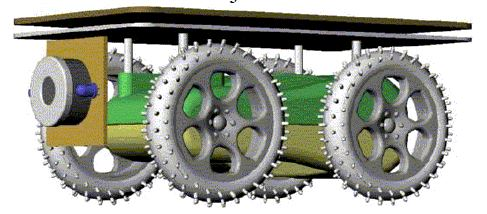
\includegraphics[width=0.5\linewidth]{images/carrito.JPG}
\caption{Carrito}
\label{fig:carrito}
\end{figure}
Se dispone del carrito de la Figura \ref{fig:carrito}, el cual posee un fototransistor y un par de leds en frente. Los leds generan radiación infraroja que se ve reflejada en la superficie que se encuentre enfrentada. Esta reflexión le da información al fototransistor sobre a qué distancia está el frente del carrito de la superficie. 

El fototransistor se encuentra encerrado en un housing con una película oscura para reducir la perturbación de la luz visible, siendo esta película transparente a la radiación infrarroja.

El carrito posee un motor de corriente continua que le permite desplazarse en una sola dirección pero en ambos sentidos dependiendo de la polaridad de la tensión entregada al motor.

Se utilizó un microcontrolador tipo Arduino como ADC para la lectura del fototransistor, cuya respuesta de tensión en función de la distancia tiene forma de gaussiana. Es decir, estando junto a la pared, la señal de salida es de aproximadamente 0V, y comienza a aumentar hasta llegar a un máximo a medida que se aleja de la pared, y luego disminuye nuevamente hasta 0V si se lo sigue alejando.

\section{Modelo del carrito}

\begin{figure}[H]
\centering
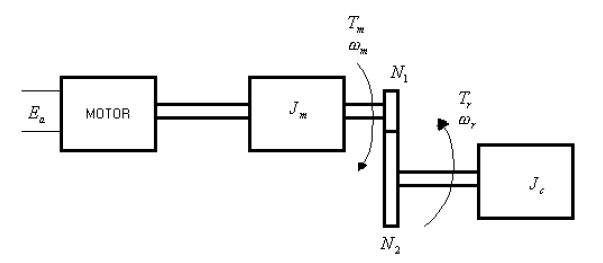
\includegraphics[width=0.7\linewidth]{images/SistemaFisico.JPG}
\caption{Representación del sistema físico}
\label{fig:carrito}
\end{figure}
Se busca encontrar la transferencia $\frac{Y(S)}{E_a(S)}$, siendo $Y(S)$ el desplazamiento lineal del carrito sobre una superficie plana. Del desarrollo y despeje provisto por la cátedra, se obtiene la función:

\[
G(S) = \frac{Y(S)}{E_a(S)} = \frac{N \cdot K_m \cdot r}{R_a \cdot J_{eq} \cdot \left( S + \frac{K_b \cdot N^2 \cdot K_m}{R_a \cdot J_{eq}} \right) \cdot S}
\]

La cual caracteriza al sistema como segundo orden con un polo en el origen.

\newpage
\section{Control PID}

El sistema realimentado con el control PID se muestra a continuación:

\begin{figure}[H]
\centering

\includegraphics[width=0.7\linewidth]{images/bloquesPID.png}
\caption{Sistema realimentado con compensador PID}
\label{fig:carrito}
\end{figure}

Donde $G(S)$ es la transferencia del carrito $\frac{Y(S)}{E_a(S)}$ (siendo la posición respecto a la tensión de alimentación del motor), y la transferencia del controlador:

\[
G_{PID}(S) = K \cdot \frac{(S+Z_1)(S+Z_2)}{S}
\]

Para aplicar el control PID, se trabaja con el primer tramo inyectivo de la respuesta del fototransistor, es decir desde 0 hasta el máximo, buscando que el carrito se mantenga a una distancia intermedia entre esos dos puntos. El valor de tensión (que depende de la distancia) se muestrea con el ADC del Arduino, y es con el cual se realimenta al sistema.\par
Para el control del motor, se utiliza la Placa Stepper para Arduino (AR-L298SHIELD), cuya implementación se trata con la librería L298.h. La señal realimentada que va al controlador PID restada a $R(S)$, se convierte luego en un valor de duty para la señal de PWM para la Placa Stepper.\par
Las constantes $K_p$, $K_d$ y $K_i$ del controlador PID se ajustaron con la metodología descripta en la sección siguiente (dado que no se conocen los valores de la planta).


\section{Método manual de ajuste}
Se ajustaron las constantes mediante el método manual:
\begin{itemize}
  \item Primero establecer $K_i=0$ y $K_d=0$. 
  \item Incrementar $K_p$ hasta que la salida oscile (es decir, el carrito presente un movimiento oscilatorio lo más armónico posible).
  \item Establecer $K_p$ a aproximadamente la mitad del valor configurado previamente.
  \item Incrementar $K_i$ hasta que el proceso se ajuste en el tiempo requerido (precaución: aumentar mucho $K_i$ puede causar la inestabilidad del sistema, ya que los polos a lazo cerrado se mueven por el lugar de raíces y puede pasar al semiplano derecho).
  \item Finalmente, incrementar $K_d$ si se necesita hasta que el lazo sea lo suficientemente rápido para alcanzar su referencia tras una variación brusca de la carga. Para el sistema bajo análisis se corresponde con, por ejemplo, tener al carrito fijo a una distancia, y de manera repentina colocar la mano delante del fototransistor, lo cual cambia abrutamente la medición de distancia.

 
\newpage
\section{Código}
\begin{lstlisting}

#include <L298N.h>
#include<PID_v1.h>

void setMotorSpeed(int s);

#define PH_EN 10
#define PH_INA 9
#define PH_INB 8
#define KP 1.4 // Valor de oscilatorio 3.2 con KD y KI en 0
#define KI 0.4
#define KD 0.2

double sp = 307; // Set point del sistema
double in = 0; // Medicion de la salida del sistmea - la realimentacion 
double out=0; // Entrada a la planta

L298N canalA(PH_EN,PH_INA,PH_INB);
PID myPID(&in, &out, &sp,KP,KI,KD, REVERSE);

void setup() {
 myPID.SetMode(AUTOMATIC);//turn the PID on
 myPID.SetOutputLimits(-255,255);
 myPID.SetSampleTime(10);//10ms de sampleo
}

void loop() {
  in = analogRead(0);
  myPID.Compute();
  setMotorSpeed(out);
  Serial.println(out);
  
}

void setMotorSpeed(int s){
  if(s>128){
    s=128;
  }else if(s<-128){
    s=-128;
  }

  // Seteo velocidad y direccion
  if(s<0){
    canalA.setSpeed(-s);
    canalA.forward();   
  }else if(s<256){
    canalA.setSpeed(s);
    canalA.backward();    
  }
}

\end{lstlisting}
 
  
\end{itemize}
\end{document}
